\documentclass{goose-article}

\usepackage{lipsum}

\title{goose-article: customized \LaTeX-article}

\author[1]{T.W.J.~de~Geus$^{*,}$}

\affil[1]{
  Physics Institute, \'{E}cole Polytechnique F\'{e}d\'{e}rale de Lausanne (EPFL) \nl
  Switzerland
}

\contact{%
  $^*$Contact: %
  \href{mailto:tom@geus.me}{tom@geus.me} %
  \hspace{1mm}--\hspace{1mm} %
  \href{http://www.geus.me}{www.geus.me}%
}

\hypersetup{pdfauthor={T.W.J. de Geus}}

\header{goose-article}

\begin{document}

\maketitle

\begin{abstract}
\noindent
\lipsum[1]

\keywords{\LaTeX-style; example}
\end{abstract}

\section{Introduction}
\lipsum[2-4] \citep{Geus10,Geus11,Geus12}

% \begin{figure}[htp]
%   \centering
%   \includegraphics[width=.5\linewidth]{figures/myoldfigures}
%   \caption{Caption here}
%   \label{fig:a}
% \end{figure}
\begin{figure}[htp]
  \centering
  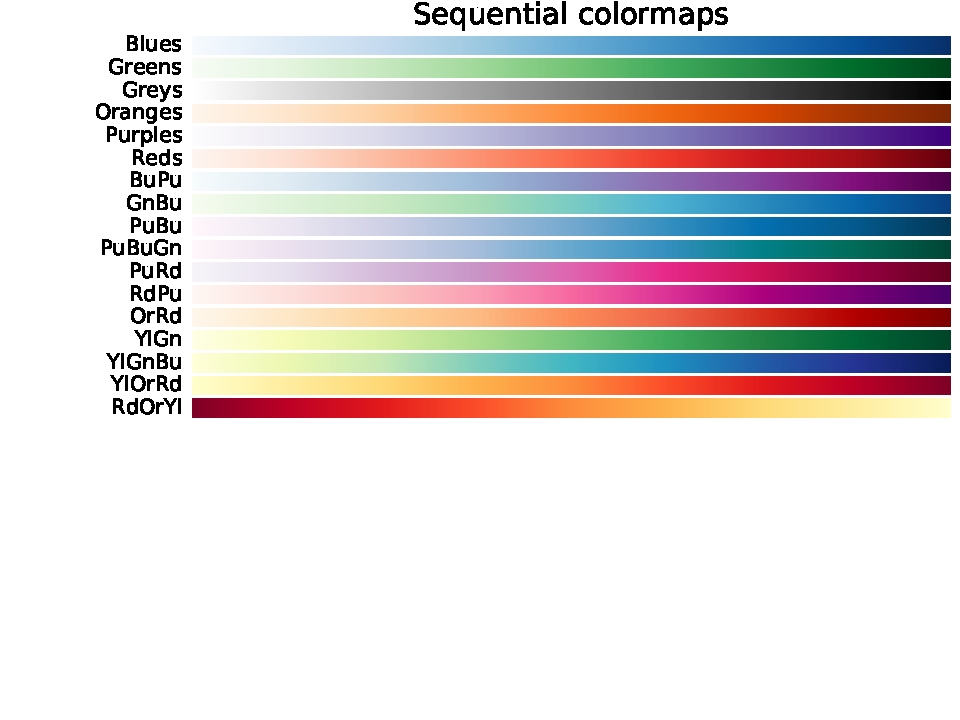
\includegraphics[width=.5\linewidth]{figures/Sequential}
  \caption{Caption here}
  \label{fig:a}
\end{figure}

\section{Body}
\lipsum[5-10] \citet{Geus13,Foo.Bar} ...

\begin{figure}[htp]
  \centering
  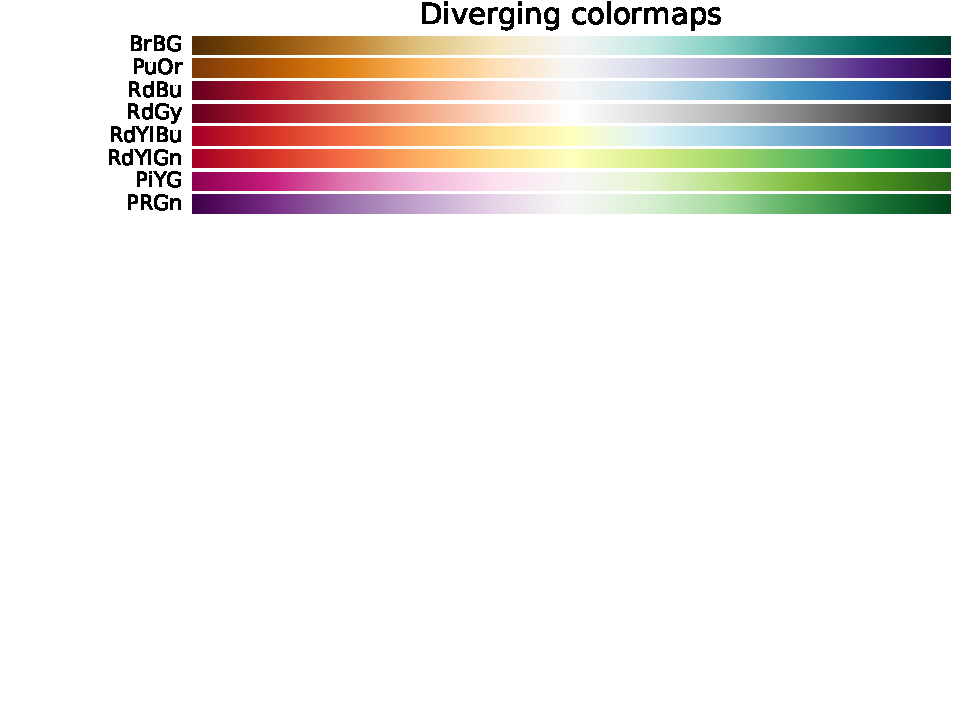
\includegraphics[width=.5\linewidth]{figures/Diverging}
  \caption{Caption here}
  \label{fig:b}
\end{figure}

\bibliography{refs}
% \bibliography{myoldrefs}

\end{document}
